\documentclass[]{article}

\usepackage{hyperref}
\usepackage{listings}
\usepackage{color}
\usepackage{caption}
\usepackage{graphicx}
\usepackage{subcaption}
\usepackage{etoolbox}

\usepackage{pgf,tikz}
\usepackage{mathrsfs}
\usetikzlibrary{arrows}

\usepackage{pgfplots}
\pgfplotsset{width=13cm,compat=1.9}

\definecolor{qqwuqq}{rgb}{0.,0.39215686274509803,0.}
\definecolor{uuuuuu}{rgb}{0.26666666666666666,0.26666666666666666,0.26666666666666666}
\definecolor{qqqqff}{rgb}{0.,0.,1.}


\definecolor{mygreen}{rgb}{0,0.6,0}
\definecolor{mygray}{rgb}{0.5,0.5,0.5}
\definecolor{mymauve}{rgb}{0.58,0,0.82}
\lstset{
    language=C++,
    captionpos=b,
    commentstyle=\color{mygreen},
    keywordstyle=\color{blue},
    stringstyle=\color{mymauve},
    frame=single,
    otherkeywords={},
}
\renewcommand{\lstlistingname}{Source Code}


\title{Planning and Navigation for a Game Bot}
\author{Giorgio Gori}

\begin{document}

\maketitle

\begin{abstract}
    Games can force players into repetitive tasks in order to obtain in-game values such as currency or experience. Virtual worlds have different rules from reality but can be automated using using robotics techniques. This paper presents a method to improve the efficiency over the state of the art by real-time path-planning using the information provided by the environment.
\end{abstract}

\section{Introduction}
% Introduction: Motivation of your problem, starting from a broad level and narrowing to your particular problem.  Brief description of the specific problem you will solve, how you will solve it, and your results (in some sense, this is an outline of the paper).
In-game values such as currency, items or experience are sought by players. Those can typically be obtained by killing computer-controlled agents in the game world. This process is repetitive, tedious, often fairly simple, and thus leads to investigating automation and robotics techniques where a piece of software is in control of the game character instead of the human player. This paper will refer to this software as the ``robot''.

In section 1 we provide an overview of the chosen game, the virtual world and the interface between game and robot. Section 2 contains the formal and informal description of the task to perform. In section 3 we will go over the current state of the art and related work in computational robotics. Section 4 contains a description of the proposed method. Section 5 contains experimental results and analysis. Finally, section 6 contains conclusions and future work.

\subsection{Game Overview}
We choose the game Guild Wars\footnote{\url{http://www.guildwars.com/}}. It is a relatively old game, released in 2005, that still has a modern interface and play style. Game areas are instanced, meaning that we can have the robot be alone with computer-controlled characters. This is good as the robot does not interfere with other players' experience and the robot only has to handle a relatively predictable world.

\subsection{Game World}
The world space is two dimensional with continuous x and y coordinates, there is no vertical axis. Coordinates and distances are in unspecified ``game units'', which have no real-life counterpart. As a general idea, a character height is approximately 100 units. 

There are two kinds of objects in the world, the first is obstacles. Those are represented as trapezoids like shown in Source Code \ref{lst:structures}. Those objects only serve as obstacles and other objects cannot move inside them. Their location is always fixed and known in advance.

The other objects are the agents, this includes the player character and any computer-controlled characters. As shown in Source Code \ref{lst:structures}, each agent has an unique ID, a position $(x, y)$ in the world and many more attributes. Agents can move freely in the world with a constant speed, as long as they don't collide with obstacles or other agents.

The character controlled by the player or by the robot is an agent with the same characteristics as any other, but for clarity in this paper we will refer to ``agents'' as all moving objects that are not the character. 

\begin{lstlisting}[caption={Game Structures}, label=lst:structures]
struct Agent {
    long id;
    float x;
    float y;
    // and more
}

struct MapTrapezoid {
    long id;
    float XTopLeft, XTopRight, YTop;
    float XBottomLeft, XBottomRight, YBottom;
}
\end{lstlisting}

\subsection{Sensors}
The game offers most of its information through a 3D interface. Human players are good at interpreting it, but a robot would need a complex computer vision system to translate the images to data such as x,y coordinates. 

Our approach instead is to read the raw data directly from the game memory. We find fixed memory addresses that hold pointers to game structures. For example we use an address that holds the pointer to the game's internal array of agents, which contains pointers to the Agent structures shows previously in Source Code \ref{lst:structures}. Declarations of those accessors are shown in Source Code \ref{lst:accessors}.

\newpage
\begin{lstlisting}[
caption={Declaration of accessors},
label=lst:accessors]
Agent* GetPlayer();
vector<Agent*> GetAgents();
vector<MapTrapezoid*> GetMap();
\end{lstlisting}

Just like with real sensors, the robot and other agents have a limited vision range. The range limitation means that each agent only has knowledge of other agents within a fixed radius. This radius is known and is equal to approximately 1000 game units for agents and 5000 game units for the robot.

\subsection{Actuators}
Human players typically move the character by clicking on the ground in the game interface. The robot could send similar input by simulating a mouse click, but the location is dependent on the camera position, zoom, etc. Instead, we can trace the call: the game will translate the click coordinates from in screen to world space and then call an internal function. We locate this internal function and the robot can then use it directly as in Source Code \ref{lst:actuators}.

\begin{lstlisting}[
caption={Declaration of Move function},
label=lst:actuators]
void Move(float x, float y);
\end{lstlisting}

\section{Problem Statement}
% Problem formulation: Describes the problem in detail, generally introducing a mathematical description of the problem.  It will also generally give some description of how you will judge the quality of your solution.
We choose a location containing a specific kind of agents. In game terms, they are very powerful spell-casters, but in the game it is possible to equip a spell-invulnerability enchantment, which means that they can only use their weak basic attacks and few protection enchantments are enough to reduce the damage taken by the robot to zero. In other words, the agents are not able to kill the robot regardless of how many or them are attacking the robot. The robot still has to maintain its protective enchantments, but that is relatively easy and outside the scope of this paper. \\

Another important observation is that the robot has to kill agents in order to collect loot. The robot is equipped with area of effect (AoE) spells, meaning that it will do the same damage to nearby agent regardless of how many there are, as long as they are nearby. Using those spells takes time, so the most efficient way to collect loot is to gather as many agents as possible, and then kill all of them at once. \\

Finally, it is important to understand the behavior of the agents. They are all computer controlled, and they are fairly predictable. Agents spawn in random locations in the world in groups of 4. After they spawn, they will each move slowly and randomly. This behavior continues until they see an enemy, and as soon as they see one, they will chase and attack it. In our case their enemy is the robot, and this is great for our purpose, as we want the agents to follow the robot. Note that their vision is shared between the group of 4, so as soon as one can see the robot, all members of the group will start chasing it. \\

We can conclude and describe the task informally as ``Group all agents in the map'', or ``Move in such a way that all agents can see the robot at least once''. \\

Formally, the problem can be described as follows: \\
Take as input a starting robot position $(S_x, S_y)$, an end position $(E_x, E_y)$ and a set $Agents = \{A_1, A_2, ..., A_n\}$ where each agent $A_i = \{id_i, x_i, y_i\}$. \\
Produce as output the shortest path $P = (p_1, p_2, ..., p_{m-1}, p_m)$ such that $p_1 = (S_x, S_y)$, $p_m = (E_x, E_y)$ and for at least one agent $A_i$ in each group, $distance(A_i, p_j) < k$ for some $p_j \in P$. \\

Agents keep moving randomly and the robot can discover new agents as it travels, so it is not enough to compute the path once and use it. Instead, at each time step the robot should compute the shortest path $P$ and move towards the next step $p_2$.

\section{Related Work}
% Background and related work: Discusses previous results in this and other fields, and how they relate to the results in this paper.
\subsection{State of the Art}
The map is known in advance and never changing, and the agents typically appear in relatively similar positions, so the state of the art robots take the easiest approach: to specify in advance a list of coordinates that the robot should visit. This approach is referred as ``Coordinate-based'' or ``Fixed-path''. The advantages of this technique are its simplicity and robustness, but the obvious disadvantage is that the robot is blind to the environment. This kind of robot will not use agent positions, and because of that, will often perform unnecessary detours or miss groups of agents.

In this paper we will provide a solution to this blindness by using computational robotics techniques to make the robot react to the environment instead.

\subsection{Related problems in Computational Robotics}
The general problem immediately looks like the Traveling Salesman Problem (TSP). TSP has widely been explored in robotics literature, for example \cite{dorigo1997ant} gives an presentation of the problem and provides an heuristic to solve it.

The TSP also has some variants that are more relevant to the problem, \cite{alatartsev2013optimizing} presents most of those variants and provides a solution to a similar problem that involves precisely visiting arbitrary shapes, the difference to this paper being that the problem is more difficult because of the arbitrary shapes, but the world is static, so computing a solution once is enough.

Two variants of TSP are particularly relevant. Generalized TSP (GTSP) involves visiting one node for every group as presented in \cite{laporte1996some} and this relates to our problem of only visiting one agent for every group. Close-Enough TSP (CETSP) consists in visiting each nodes by going to the neighborhood of the node, similar to visiting a circle centered at each node as shown in \cite{mennell2009heuristics}. CETSP relates to our problem since we also only need to move within a set radius to the node. CETSP heuristic also often rely on a secondary problem, the touring of a sequence of circles as described in \cite{chou2012shortest}.

Overall, our problem is a combination of GTSP and CETSP.

\section{Proposed Method}
The proposed method consists in three different components, first of all we cluster agents in groups of 4, then we compute shortest path between the groups using a Generalized Traveling Salesman Problem algorithm, and then we make an optimization pass.

\subsection{Clustering}
Groups of agents are fixed and set when they are created. We discovered that the agents of a group are created very close to each other, and start moving as soon as they are in vision of the robot. This allows the robot to perform a very simple and yet robust clustering. 

At each time step the robot makes a list of all unclustered agents. If it can find 4 agents all within a fixed distance (experimentally set to 750 units) it will save them as a group. This process is performed in a greedy way until no clusters can be created. As soon as a group can see the robot it will start following, we don't need to consider it any more, so we remove it. This will save time later in the path planning. The life cycle of a group is shown in Figure \ref{fig:groups}.

\begin{figure*}[h]
\begin{subfigure}{0.19\textwidth}
    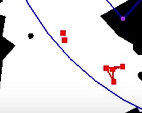
\includegraphics[width=\linewidth]{pics/cluster1.png}
    \caption{}
\end{subfigure}
\begin{subfigure}{0.19\textwidth}
    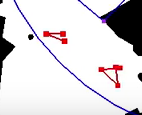
\includegraphics[width=\linewidth]{pics/cluster2.png}
    \caption{}
\end{subfigure}
\begin{subfigure}{0.19\textwidth}
    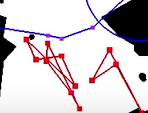
\includegraphics[width=\linewidth]{pics/cluster3.png}
    \caption{}
\end{subfigure}
\begin{subfigure}{0.19\textwidth}
    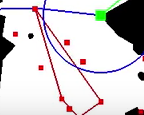
\includegraphics[width=\linewidth]{pics/cluster4.png}
    \caption{}
\end{subfigure}
\begin{subfigure}{0.19\textwidth}
    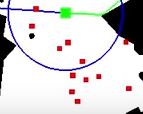
\includegraphics[width=\linewidth]{pics/cluster5.png}
    \caption{}
\end{subfigure}
\caption{Agents are represented by red squares and red lines connecting them represent groups. Two groups are created in (a) and (b), then they start moving randomly (c) along with a third group. Finally, the robot is seen by two of the three groups in (d) and they are removed. In (e) all groups saw the robot and were removed.}
\label{fig:groups}
\end{figure*}

\subsection{Generalized Traveling Salesman Problem}
Once we have the groups, we need to compute in which order to visit them. We do that with a simple nearest neighbor approach. We construct a list of clusters, add the nearest to the path while removing it from the list, and repeat until the list is empty. 

The main downside of the nearest neighbor algorithm is poor results towards the end of the tour, when most nodes are visited and hops become very long. However, we mostly care about the starting part of the tour, since that is where the robot will move. Towards the end of the path the data is also unstable, since we add groups as we see new agents. Nearest neighbor approach gives us stability where we need it the most at the begin of the tour, and it is a simple and fast method.

It may seem counterintuitive and unnecessary to compute the whole path with nearest neighbor and then only move towards the first neighbor, however computing the full path is important for the optimization pass below.

\subsection{Path optimization}
We perform two passes of path optimization.

First of all, we select the best agent to visit within every cluster. The nearest neighbor path generated in the last step favors agents close to the robot, but those are not necessarily the best. For every group in the path, we compute for every agent the distance from the previous group, to the agent, to the next group. The agent paired with the smallest sum of distances is selected.

The second step involves computing the final location to visit for each agent. Up until now, we used agents as nodes in the path, but the robot does not need to visit the agent, it only needs to be seen by them, or in other words, to be within a fixed distance to them. We use the 2-dimensional specialization of the 3-dimensional line intersection algorithm from \cite{Goldman:1990:ITL:90767.90838}. There are two possible scenarios, shown in Figure \ref{fig:opt}, either the robot needs to make a detour to be seen by the Agent or it can just move straight. We use the above algorithm to detect the scenario and to find the point to visit. Finally we check if the selected point is valid in the navigation map, meaning it is not inside an obstacle, in case it is not valid, we revert this step and just use the agent position as destination.

\begin{figure}
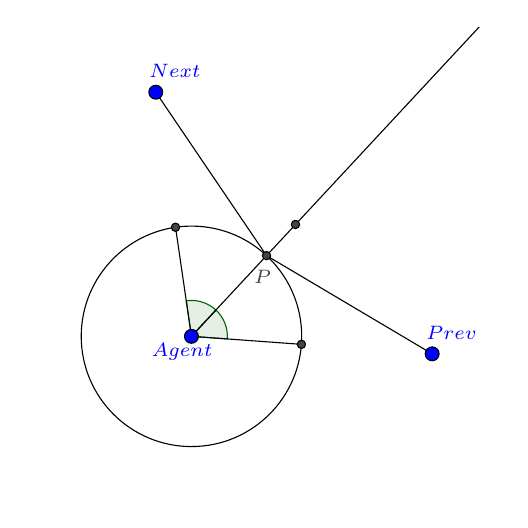
\begin{tikzpicture}[line cap=round,line join=round,>=triangle 45,x=2.0cm,y=2.0cm]
\clip(2.2,-1.) rectangle (5.2,2.);
\draw [shift={(3.24,0.04)},color=qqwuqq,fill=qqwuqq,fill opacity=0.1] (0,0) -- (47.07744156565525:0.2280415580347225) arc (47.07744156565525:98.31524005752445:0.2280415580347225) -- cycle;
\draw [shift={(3.24,0.04)},color=qqwuqq,fill=qqwuqq,fill opacity=0.1] (0,0) -- (-4.160356926214376:0.2280415580347225) arc (-4.160356926214376:47.07744156565525:0.2280415580347225) -- cycle;
\draw(3.24,0.04) circle (1.4cm);
\draw [domain=3.24:5.2] plot(\x,{(-1.64173105437033--0.5125923805161493*\x)/0.47670646254984517});
\draw (4.7683761491495575,-0.07117379283739354)-- (3.7167064625498454,0.5525923805161493);
\draw (3.7167064625498454,0.5525923805161493)-- (3.0134072547100224,1.5903498016367272);
\draw (3.24,0.04)-- (3.138766420667486,0.7326411498139048);
\draw (3.24,0.04)-- (3.9381554385161692,-0.010783694925548815);
\begin{scriptsize}
\draw [fill=qqqqff] (3.24,0.04) circle (2.5pt);
\draw[color=qqqqff] (3.1806377306021525,-0.05915080148109428) node {$Agent$};
\draw [fill=qqqqff] (4.7683761491495575,-0.07117379283739354) circle (2.5pt);
\draw[color=qqqqff] (4.890949415862571,0.06247136280409072) node {$Prev$};
\draw [fill=qqqqff] (3.0134072547100224,1.5903498016367272) circle (2.5pt);
\draw[color=qqqqff] (3.1350294189952077,1.7271747364575603) node {$Next$};
\draw [fill=uuuuuu] (3.138766420667486,0.7326411498139048) circle (1.5pt);
\draw [fill=uuuuuu] (3.9381554385161692,-0.010783694925548815) circle (1.5pt);
\draw [fill=uuuuuu] (3.7167064625498454,0.5525923805161493) circle (1.5pt);
\draw [fill=uuuuuu] (3.90063334377932,0.7503650672677357) circle (1.5pt);
\draw[color=uuuuuu] (3.6922945265829397,0.41973647039182166) node {$P$};
\end{scriptsize}
\end{tikzpicture}
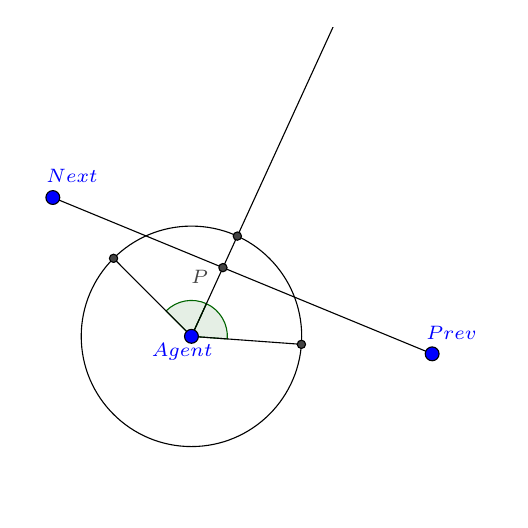
\begin{tikzpicture}[line cap=round,line join=round,>=triangle 45,x=2.0cm,y=2.0cm]
\clip(2.2,-1.) rectangle (5.2,2.);
\draw [shift={(3.24,0.04)},color=qqwuqq,fill=qqwuqq,fill opacity=0.1] (0,0) -- (65.40167379068055:0.2280415580347225) arc (65.40167379068055:134.9637045075748:0.2280415580347225) -- cycle;
\draw [shift={(3.24,0.04)},color=qqwuqq,fill=qqwuqq,fill opacity=0.1] (0,0) -- (-4.160356926214376:0.2280415580347225) arc (-4.160356926214376:65.40167379068055:0.2280415580347225) -- cycle;
\draw(3.24,0.04) circle (1.4cm);
\draw (2.3596881216771513,0.9214278980682097)-- (4.7683761491495575,-0.07117379283739354);
\draw [domain=3.24:5.2] plot(\x,{(-2.050519956855312--0.6364737886750595*\x)/0.291377961297032});
\draw (3.24,0.04)-- (2.7453389070097796,0.5352882020417205);
\draw (3.24,0.04)-- (3.9381554385161692,-0.010783694925548815);
\begin{scriptsize}
\draw [fill=qqqqff] (3.24,0.04) circle (2.5pt);
\draw[color=qqqqff] (3.1806377306021525,-0.05915080148109428) node {$Agent$};
\draw [fill=qqqqff] (4.7683761491495575,-0.07117379283739354) circle (2.5pt);
\draw[color=qqqqff] (4.890949415862571,0.06247136280409072) node {$Prev$};
\draw [fill=qqqqff] (2.3596881216771513,0.9214278980682097) circle (2.5pt);
\draw[color=qqqqff] (2.4813102859623366,1.0582528328890428) node {$Next$};
\draw [fill=uuuuuu] (2.7453389070097796,0.5352882020417205) circle (1.5pt);
\draw [fill=uuuuuu] (3.9381554385161692,-0.010783694925548815) circle (1.5pt);
\draw [fill=uuuuuu] (3.531377961297032,0.6764737886750596) circle (1.5pt);
\draw [fill=uuuuuu] (3.4397566408602396,0.4763400219267541) circle (1.5pt);
\draw[color=uuuuuu] (3.2922945265829397,0.41973647039182166) node {$P$};
\end{scriptsize}
\end{tikzpicture}
\caption{The two cases of position optimization, Left: The robot needs to make a detour to $P$ to be seen by the Agent. Right: it can just go straight.}
\label{fig:opt}
\end{figure}

\newpage
\section{Results}
% This section typically includes examples of the problem and their solution.  In empirical papers (eg: papers that are not theoretical) you will demonstrate here that you solved the problem, and analyze the quality of the solution.
One instance of the problem consists in loading a new map and performing the task of grouping the enemies. We record the time starting the timer when the map is loaded and stopping it when all agents are around the player character. We also considered the number of missed or lost agents. Finally, we noted failure, which can be caused by getting trapped by agents and being unable to move or by failing to periodically use the required enchantments and getting killed by the agents.

The player character is controlled by four different test subjects: an expert human with experience and knowledge of game mechanics, a beginner human with little knowledge of game mechanics and experience of the task, the state of the art coordinate-based bot, and our proposed approach. We perform 10 trials for each subject. We allow for some practice time to the human subject before the 10 test trials.

\begin{figure}[h]
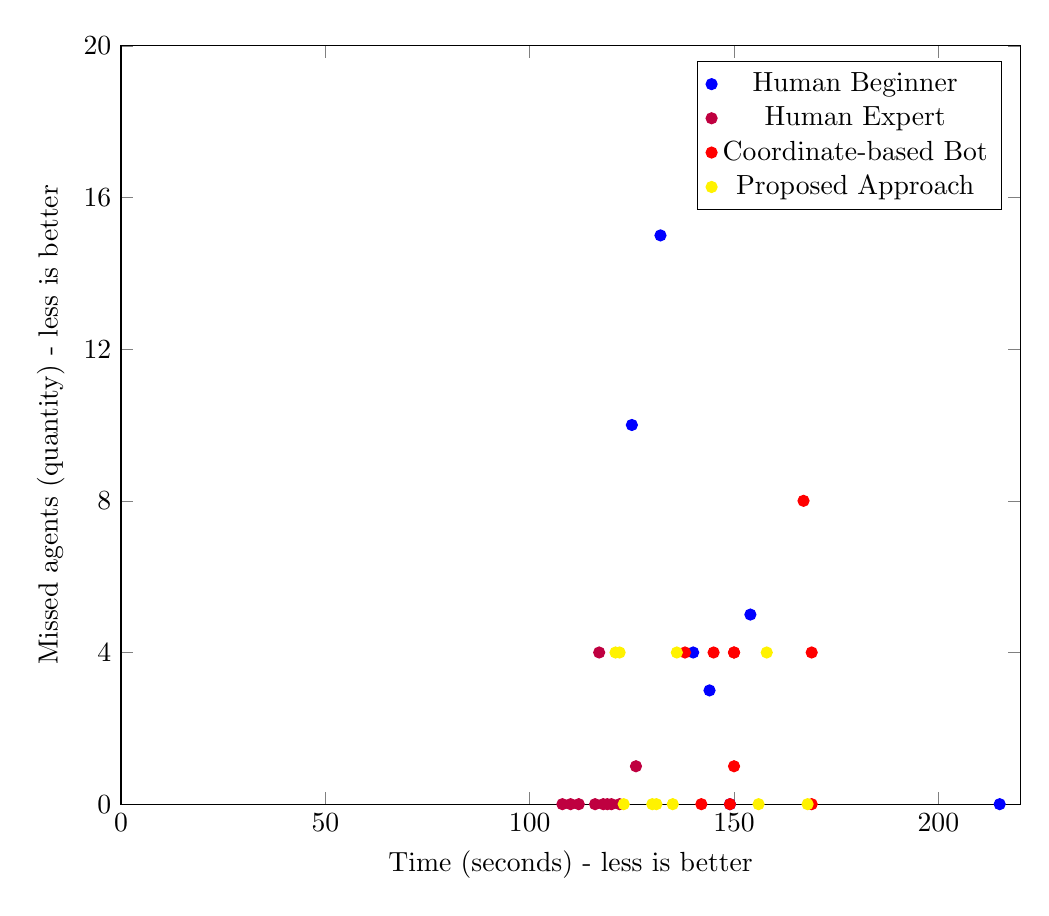
\begin{tikzpicture}
\begin{axis}[
%title=Plot of successful trials, 
xlabel=Time (seconds) - less is better,
ylabel=Missed agents (quantity) - less is better,
xmin=0, xmax=220,
ymin=0, ymax=20,
xtick={0, 50, 100, 150, 200},
ytick={0, 4, 8, 12, 16, 20},
]
\addplot[only marks, mark=*, color=blue]
coordinates{(215,0)(140,4)(150,19)(125,10)(132,15)(149,0)(144,3)(154,5)};
\addplot[only marks, mark=*, color=purple]
coordinates{(116,0)(110,0)(118,0)(117,4)(120,0)(122,0)(108,0)(119,0)(126,1)(112,0)};
\addplot[only marks, mark=*, color=red]
coordinates{(142,0)(167,8)(150,4)(138,4)(145,4)(169,0)(169,4)(150,4)(149,0)(150,1)};
\addplot[only marks, mark=*, color=yellow]
coordinates{(156,0)(122,4)(121,4)(131,0)(168,0)(130,0)((123,0)(135,0)(136,4)(158,4)};
\legend{Human Beginner, Human Expert, Coordinate-based Bot, Proposed Approach}
\end{axis}
\end{tikzpicture}
\caption{Plot of the different test trials. Different colors denote different test subjects as noted in the legend. The axis show time and amount of missed agents, in both axis less is better. The human beginner is missing three data points since those runs were fails.}
\label{results1}
\end{figure}

\begin{table}[h]
\begin{tabular}{c|c|c|c|c}
    & Average Time (seconds) & Average Missed Agents & Fails \\ \hline
    Novice Human & 151 & 7.0 & 3 \\
    Expert Human & 117 & 0.5 & 0 \\
    Coordinate-based & 153 & 2.9 & 0 \\
    Proposed Approach & 138 & 1.6 & 0 \\
\end{tabular}
\caption{Summary of the trial runs}
\label{results2}
\end{table}

\newpage
\subsection{Discussion}
% This section would draw conclusions based on the results, and mention any limitations inherent in the methodology and / or apparent in the results.
We show in Figure \ref{results1} the plot of each test trial. In this plot we are mostly looking for patterns of consistency and outliers. It is interesting to note how the proposed approach (yellow dots) yields generally good results, however there are three strong outliers with a much higher time than the others. The Coordinates-based bot performs consistently time-wise, but often misses a few agents. The ``Human Beginner'' is interesting in the fact that it is the most inconsistent: it can be relatively fast but miss a lot, or be really slow, and can still perform on par with the coordinate-based bot.

Table \ref{results2} is a summary of the runs and yet again gives a similar view on the performance of the different test subject. We can see how in average the Human Expert is the fastest, the Proposed Approach is about 20 seconds slower than that, and the Coordinate-based state of the art is an additional 15 seconds slower. The Human Novice is similar to the Coordinate-based bot in terms of time, but misses a lot more agents in average and can also fail runs.

The main limitation of those results is their number, since we performed only 10 trials for each subject.

\section{Conclusion and Future Work}
% What did you do, and what still needs to be done?
As shown by our results, we implemented a path planning method which can outperform the state of the art. Our method can perform better than a human but can't reach the consistency and speed of a experienced player. The main issue is consistency time-wise usually caused by the robot getting stuck between agents. Future work will focus on obtaining more consistency, in order to do so the bot should not only perform the existing long-term path planning but also short term path planning to avoid getting stuck by agents and terrain.

\section{References}

\patchcmd{\thebibliography}{\section*{\refname}}{}{}{}
\bibliographystyle{plain}
\bibliography{report}


\end{document}
